%	!Mode::"UTF-8"
%	本模板设置改自北京大学交叉学院 王宇哲学长和北京大学化学与分子工程学院 王应泽同学的分享,特此感谢!
%	模板制作:北京大学化学与分子工程学院 王梓涵
%	Email:2100011837@stu.pku.edu.cn
%	本模板仅适用于北京大学物理化学实验报告,其他学校请自行修改
%	吐槽:Latex用于写物化实验报告还是过于繁琐了,不过还是比Word好用多了(๑•̀ㅂ•́)و✧ (此吐槽由copilot自动生成,模板作者认为word更好用)
%	本模板仅供交流学习使用,不可用作商业用途。

\documentclass[12pt]{article}

%	页面设置
\usepackage{geometry}
\geometry{left=2.5cm, right=2.5cm, top=2.5cm, bottom=2.5cm}
\usepackage{graphicx}
\usepackage{ctex}
\usepackage{fontspec}
\usepackage{setspace}
\usepackage[usenames,dvipsnames]{xcolor}
\usepackage{titlesec}

%	字体设置
\setmainfont{Times New Roman}
\setCJKmainfont{SimSun}
\setCJKsansfont{SimHei}

%	表格设置\
\usepackage{array,colortbl}
\usepackage{makecell}
\newcommand{\addcell}[2][4]{\makecell{\zihao{#1}\textsf{#2}}}
\usepackage{titlesec}
\usepackage{booktabs}
\usepackage{ragged2e} 
\usepackage{multirow}
\usepackage{tabularx}

% 网址设置
\usepackage{hyperref}
\hypersetup{hidelinks,
	colorlinks=true,
	allcolors=black,
	pdfstartview=Fit,
	breaklinks=true}


%	设置图注、表注
\usepackage{caption}
\usepackage{bicaption}
\captionsetup{labelsep=quad, font={small, bf}, skip=2pt}
\DeclareCaptionOption{english}[]{
    \renewcommand\figurename{Fig.}
    \renewcommand\tablename{Table}
}
\captionsetup[bi-second]{english}

%	设置页眉
\usepackage{fancyhdr}
\usepackage{xpatch}
\pagestyle{fancy}
\fancypagestyle{preContent}{
    	\fancyhead[L]{\zihao{-5} 物理化学实验}
    	\fancyhead[C]{\zihao{-5} 实验十一\ \ 紫外可见吸收光谱仪搭建与量子一维势阱方程的验证}
    	\fancyhead[R]{\zihao{-5} 2100011837\ 王梓涵}
		\renewcommand{\headrulewidth}{2pt}
		\renewcommand{\footrulewidth}{1pt}
		\xpretocmd\headrule{\color{BrickRed}}{}{\PatchFailed} % 设置页眉分割线颜色
		\xpretocmd\footrule{\color{BrickRed}}{}{\PatchFailed} % 设置页脚分割线颜色
}
\pagestyle{preContent}



%	设置首页页眉及取消首页页脚 若不需要首页页眉 请注释掉下列内容
\fancypagestyle{plain}{
	\fancyhead[L]{\zihao{-5} 物理化学实验}
    \fancyhead[C]{\zihao{-5} 实验十一\ \ 紫外可见吸收光谱仪搭建与量子一维势阱方程的验证}
	\fancyhead[R]{\zihao{-5} 2100011837\ 王梓涵}
	\cfoot{}
}

%	设置标题格式
\titleformat*{\section}{\color{Mahogany}\zihao{4}\sffamily}
\titleformat*{\subsection}{\zihao{-4}\sffamily}
\titleformat*{\subsubsection}{\zihao{-4}\sffamily}
\titlespacing*{\section}{0pt}{10pt}{10pt}
\titlespacing*{\subsection}{0pt}{10pt}{5pt}
\titlespacing*{\subsubsection}{0pt}{10pt}{5pt}


%	设置引用格式(ACS格式规范)
%	注意:请安装JabRef
%	JabRef使用参考:https://blog.csdn.net/weixin_44191286/article/details/85698921
\usepackage[super,round,comma,compress]{natbib}

%	数学公式增强
\usepackage{amsmath}
\usepackage{amssymb}

%	单位与数学式
\usepackage{siunitx}

% 其他添加
\usepackage[version=4]{mhchem}

%	设置封面
\begin{document}
    % 标题页
    \begin{titlepage}
    	% 页眉
    	\thispagestyle{plain}
        % 校徽图片
        \begin{figure}[h]
            \centering
            \includegraphics{pku.png}
        \end{figure}
        \vspace{24pt}
        % 标题
        \centerline{\zihao{-0} \textsf{\textcolor{Mahogany}{物理化学实验报告}}}
        \vspace{40pt} % 空行
        \begin{center}
            \begin{tabular}{cp{14.1cm}}
                % 题目
                \addcell[2]{题目:} & \addcell[3]{紫外可见吸收光谱仪搭建与量子一维势阱方程的验证} \\
                \cline{2-2}
            \end{tabular}
        \end{center}
        \vspace{20pt} % 空行
        \begin{center}
            \doublespacing
            \begin{tabular}{cp{5cm}}
                % 姓名
                \addcell{姓\phantom{空格}名:\ } & \addcell{王梓涵} \\
                \cline{2-2}
                % 学号
                \addcell{学\phantom{空格}号:\ } & \addcell{2100011837}\\
                \cline{2-2}
                % 组别
                \addcell{组\phantom{空格}别:\ } & \addcell{22组} \\
                \cline{2-2}
                % 实验日期
                \addcell{实验日期:\ } & \addcell{2023.10.19}\\
                \cline{2-2}
                % 室温
                \addcell{室\phantom{空格}温:\ } & \addcell{294.95\ K}\\
                \cline{2-2}
                % 大气压强
                \addcell{大气压强:\ } & \addcell{101.28\ kPa}\\
                \cline{2-2}
            \end{tabular}
            \begin{tabular*}{\textwidth}{c}
                \\ % 这是空行
                \\ % 这是空行
                \\ % 这是空行
                \hline % 分割线
            \end{tabular*}
        \end{center}
        % 摘要
        \textsf{\textcolor{BrickRed}{摘\ \ 要}}\ \  \ 本实验利用实验室提供的部件搭建了紫外可见吸收光谱仪,利用氘灯对光谱仪进行了调试和标定;用光谱仪测定了同一物质($A3$)不同浓度溶液的吸收光谱,拟合了工作曲线,测验了Lambert-Beer定律的浓度适用范围,并对比了使用氘灯光源和卤钨灯光源的差异;本实验还测量了多个共轭分子的吸收光谱,计算了各分子的摩尔吸光系数$\varepsilon$;并与用一维势阱模型和Gaussian程序对各分子的模拟计算比较,验证了一维势阱模型。
        \\
        \\
        % 关键字
        \textsf{\textcolor{BrickRed}{关键词}}\ \ 紫外可见吸收光谱仪;一维势阱模型;β-胡萝卜素 ;Lambert-Beer定律;氘灯;卤钨灯
    \end{titlepage}

    \section{引言}
		\subsection{实验目的}
			本实验的实验目的主要有以下几点\citealp{physchemlab}:\par
			\ \ \ \ \ \ \ \ 1. 了解量子力学一维势阱模型。\par
			\ \ \ \ \ \ \ \	2. 了解紫外光谱仪的原理和构成。\par
			\ \ \ \ \ \ \ \	3. 学习紫外可见光谱的搭建和调试。\par
			\ \ \ \ \ \ \ \	4. 验证Lambert-Beer定律并观察其使用范围。\par
			\ \ \ \ \ \ \ \	5. 验证量子一维势阱模型。\par
		\par
			\subsection{实验原理和实验方法}
				实验原理和实验方法在实验预习报告中如\textbf{图1}所示: \par
		\begin{figure}[h]
			\centering
			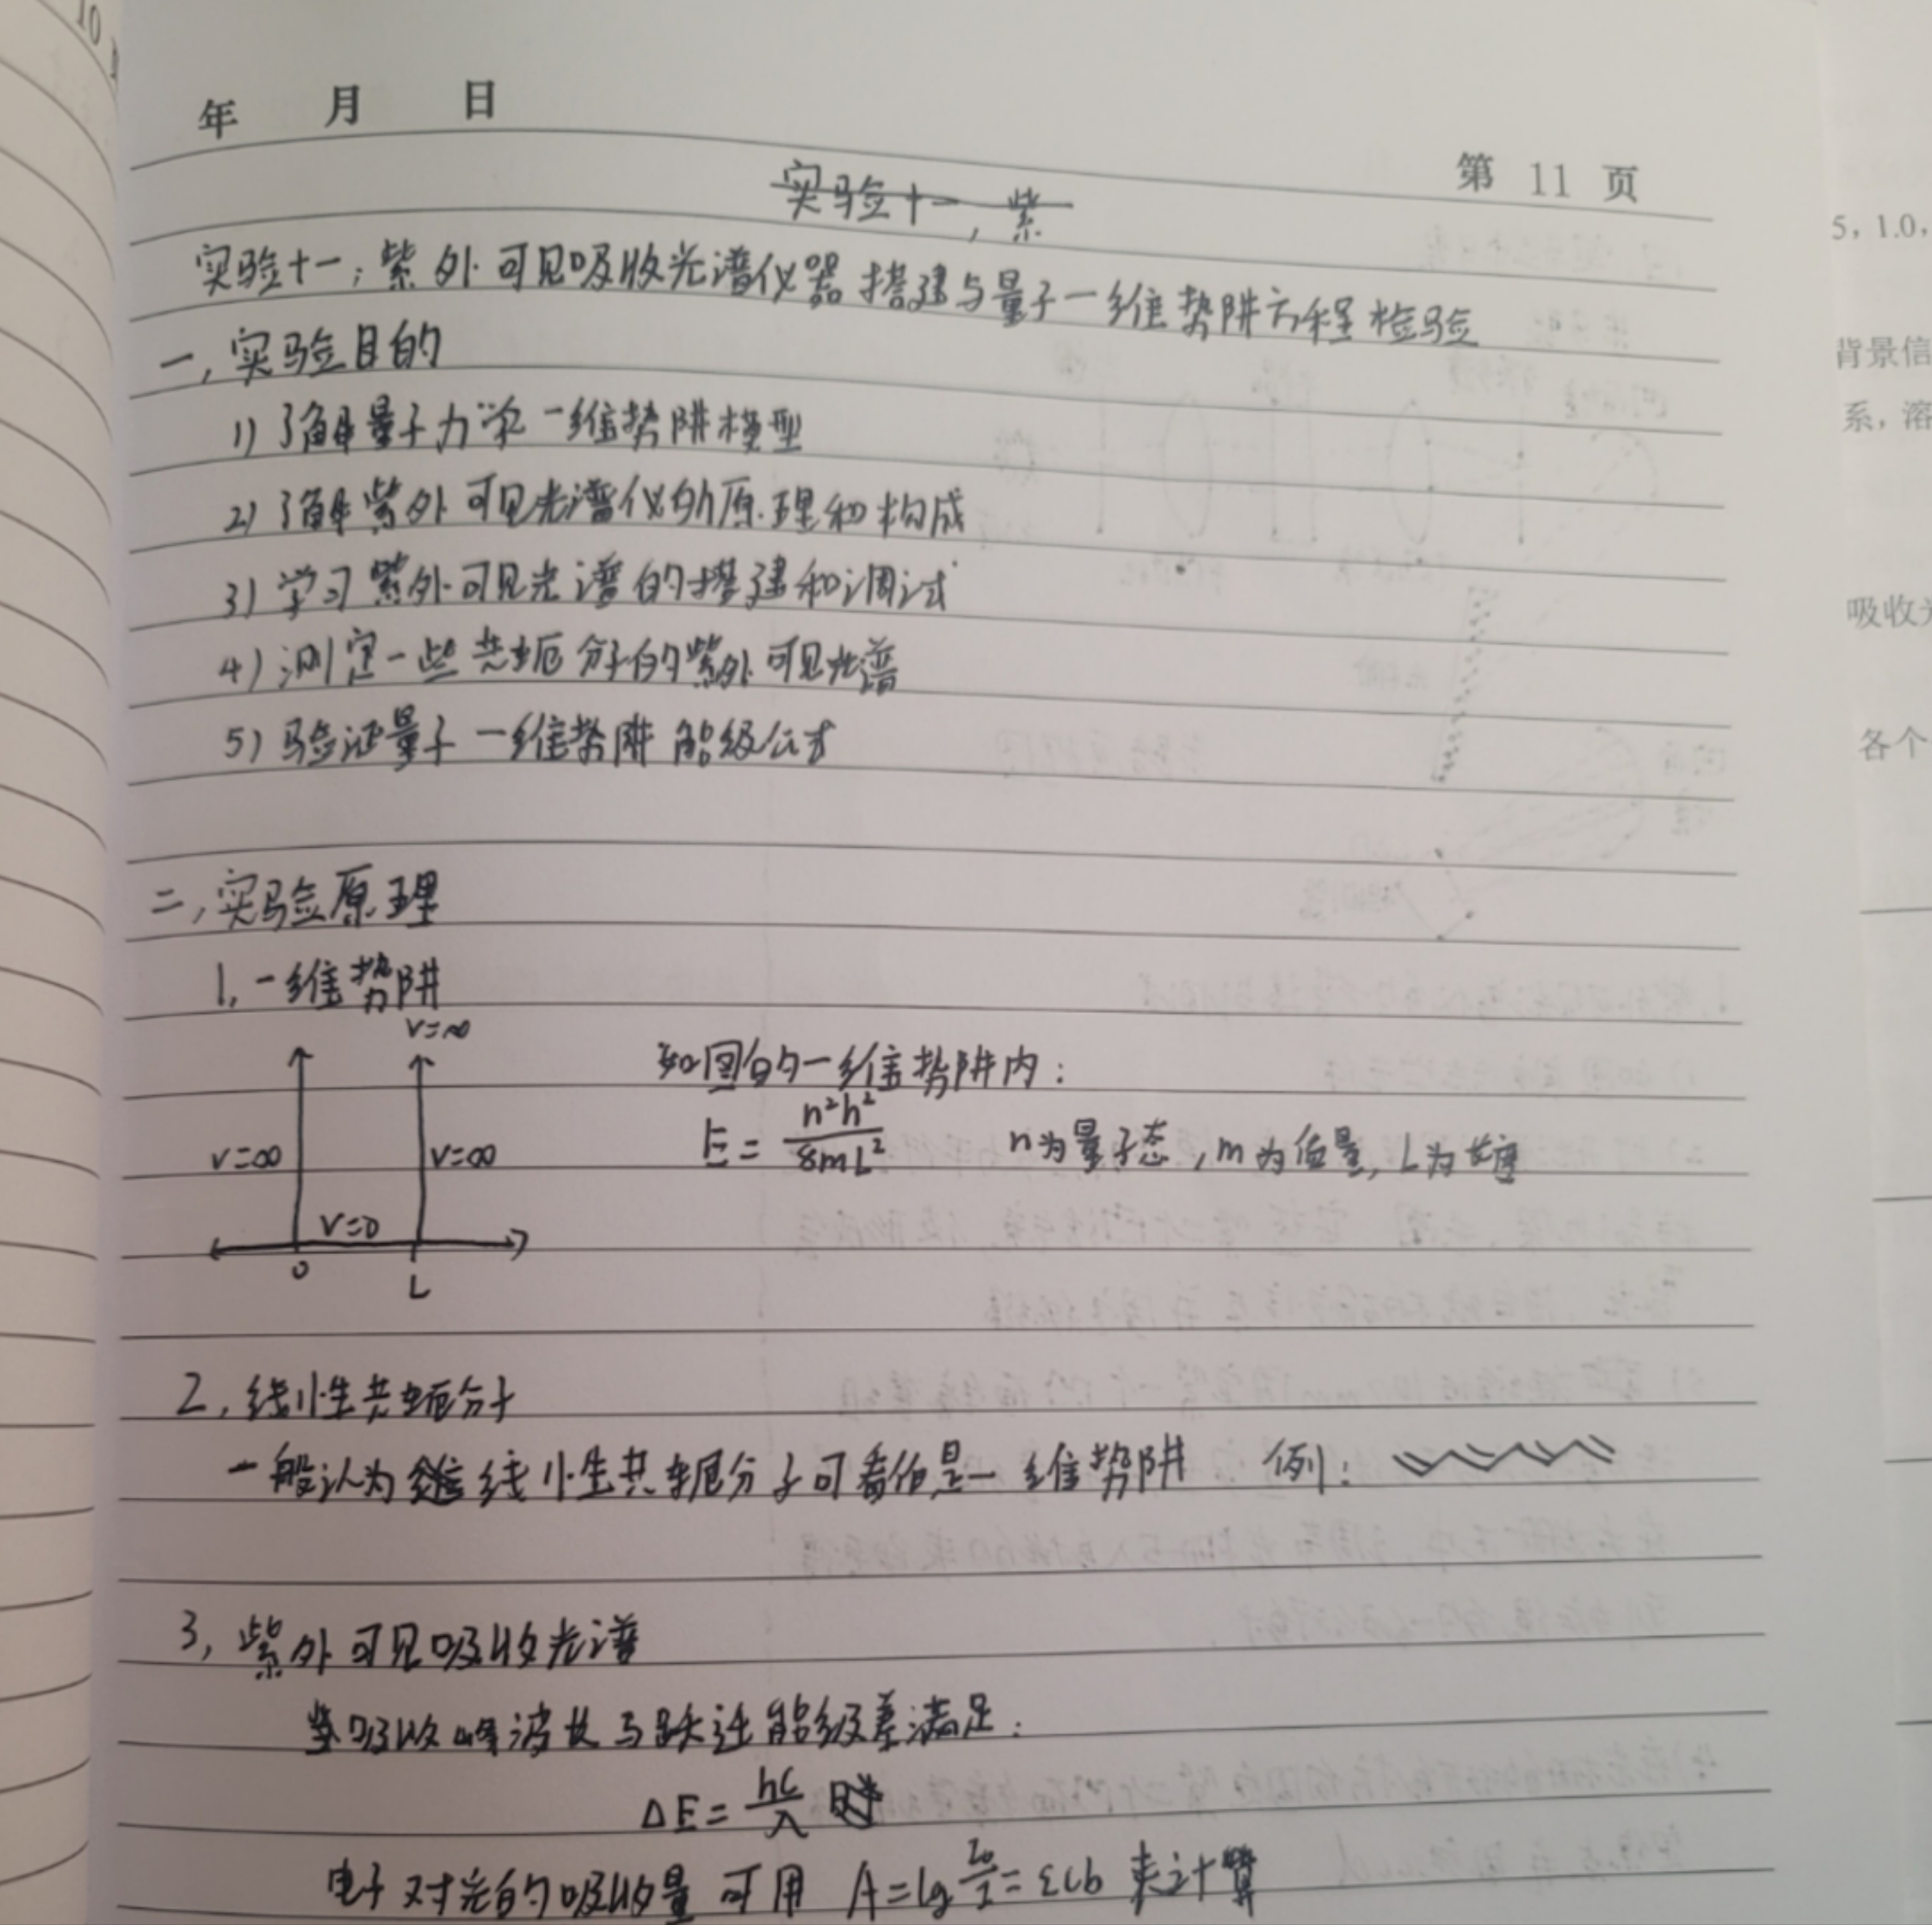
\includegraphics[width=0.8\textwidth]{1.png}
			\bicaption{实验预习报告的实验原理部分}{The principle part of the experiment in the experiment preview report}
		\end{figure}

	     
    \section{实验部分}
    	\subsection{仪器和试剂}
    		仪器:\ \  光源,光阑,平凸透镜(2个),样品池架,样品池(2个),狭缝,凹面镜(2个),光栅,ccd检测器,光学平台(面包板),
			光学元件架,光学支杆套件,遮光器材,安装工具。\par
			试剂:\ \  6种共轭分子的乙醇溶液,乙醇。具体的共轭分子详见\textbf{图2}\par
    	\par
		\begin{figure}[h]
			\centering
			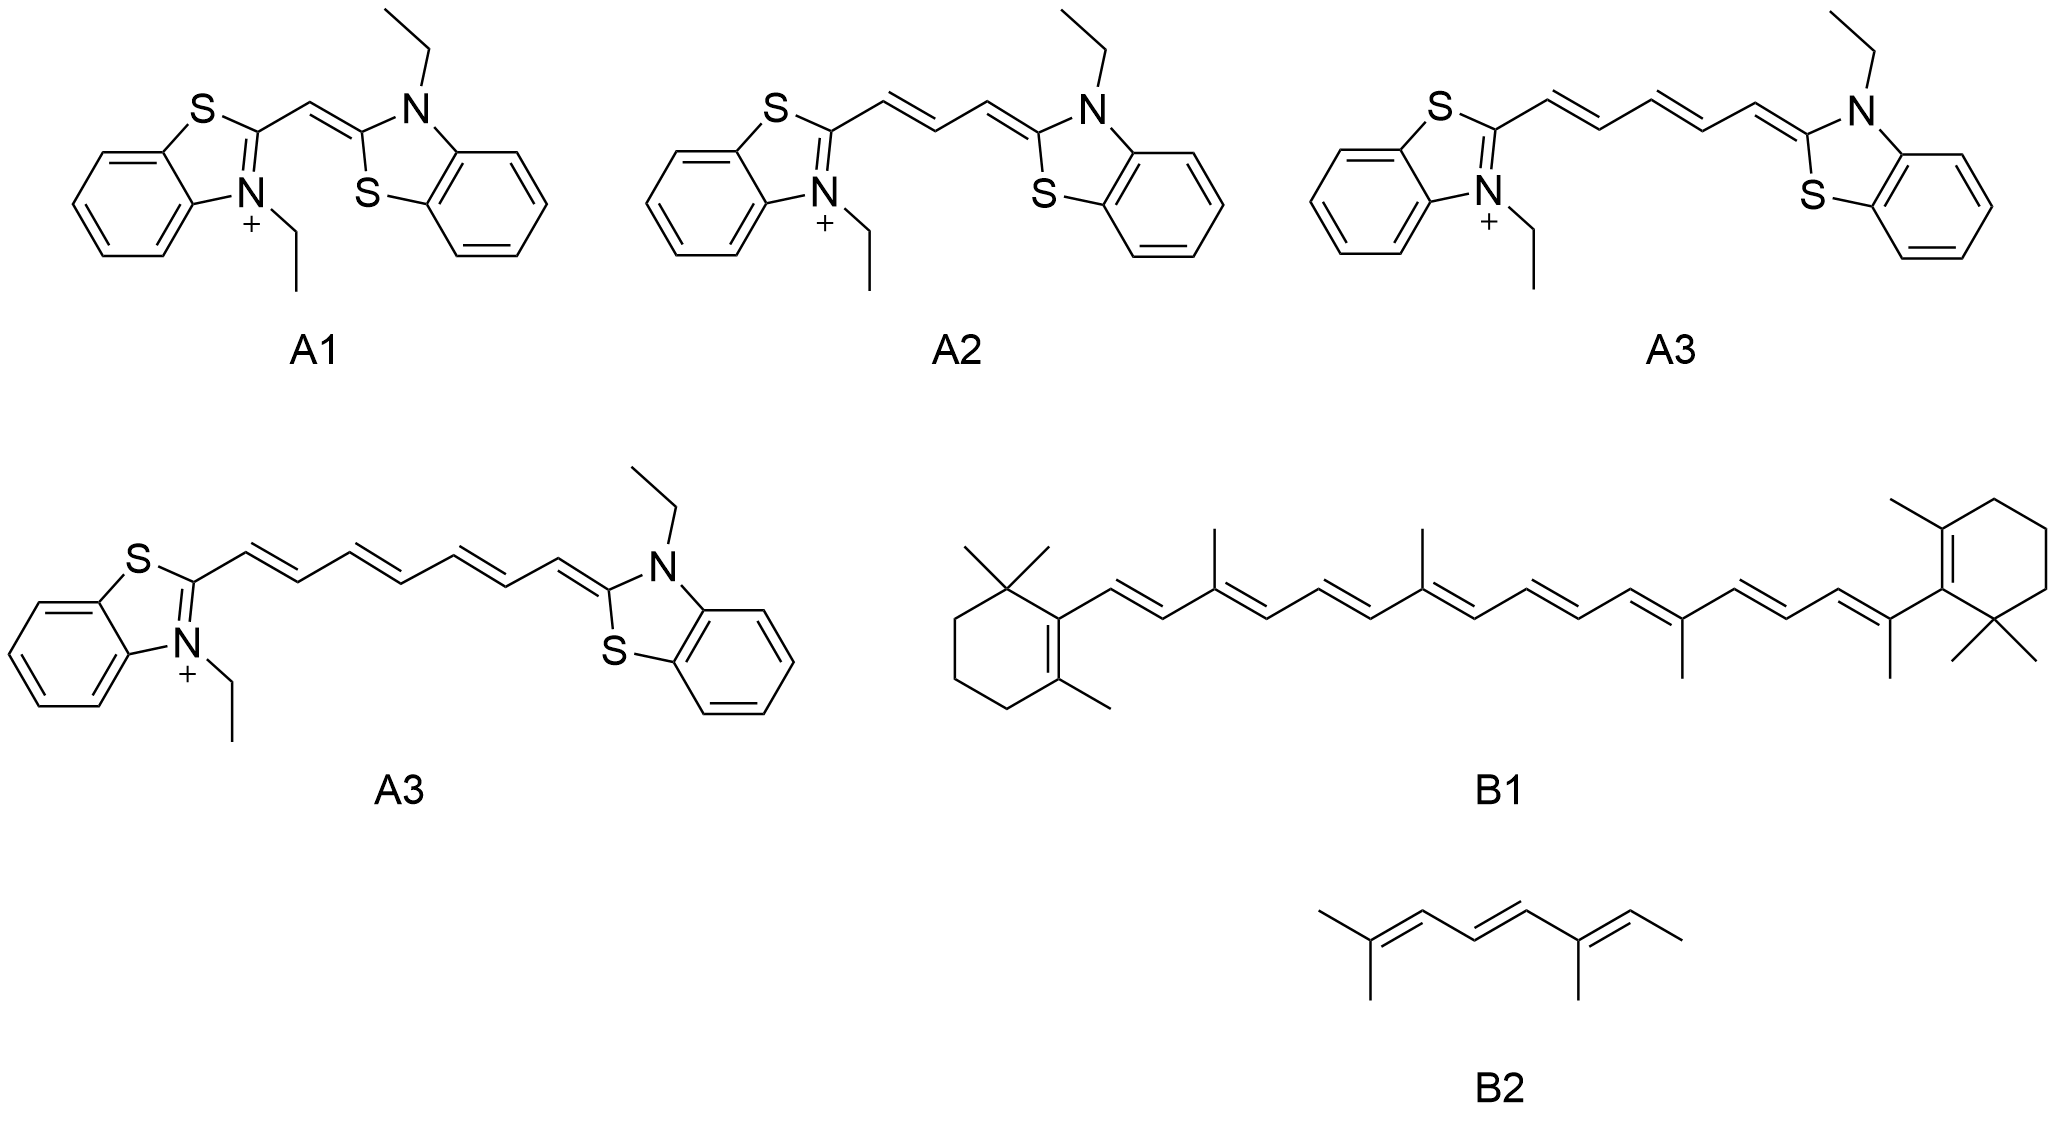
\includegraphics[width=0.8\textwidth]{2.png}
			\bicaption{6种共轭分子的结构}{Structures of 6 conjugated molecules}
		\end{figure}
			\par
    	 \subsection{实验内容\citealp{physchemlab}}
			\subsubsection{紫外可见光谱仪的搭建}
			首先将各个光学元件固定在元件架中,保证各元件和光源在同一高度。打开氘灯电源,将凸透镜套组固定在光源左侧约$75{\rm\ \ mm}$处,调整凸透镜的位置,使透射光成为平行光,即移动光屏光斑大小不变。\par
			在凸透镜后适当的位置固定样品池架,并在光源和凸透镜之间安装光阑,使样品池获得合适的光斑;在样品池后适当位置安装第二个凸透镜套组,使光束形成会聚光,将可调狭缝固定于此处。\par
			在狭缝后顺光方向约$100{\rm\ \ mm}$处固定第一个凹面镜套组,使反射光与入射光成一小夹角,且反射光近似于平行光(移动光屏光斑大小不变,实际操作中很难只能做到大概);沿反射光方向合适位置安装光栅套组,令光照在光栅的合适位置,避开划痕和污渍(ps:上一组同学将光栅的镜面直接贴到了胶布上导致我们的光栅全是划痕和污渍orz);反复调节光栅与入射光之间的夹角,用实验室提供的光屏观察分光方向,直至得到较强的一级衍射。\par
			在光栅的一级衍射方向上固定第二个凹面镜套组,用光屏确定反射光焦点位置,将ccd大概放置在此处;调整光栅与第二个凹面镜的距离,使凹面镜和ccd尽量接收到全部光谱范围($200\sim800 \ \ {\rm nm}$,即红光至蓝光占受光面积的$3/5$),但实际上由于ccd的尺寸限制,只能接收到部分的光因此需在测量中调整ccd位置\par
			用实验室提供的纸板将狭缝及之后的光路仔细遮光,并在狭缝前的纸板上开一小孔,以便光线射入;再用纸板和遮光布将光谱仪罩好。
			\subsubsection{光谱仪的标定}
			打开氘灯光源,打开电脑,连接好ccd,运行ccd控制软件,扫描光源谱图,在线调整光栅之后光路,对ccd的位置进行微调,观察分辨率的改善;观察到各特征峰足够明显时,保持光栅之后光路和ccd的位置不动,找到氘灯各个特征峰。\par
			利用氘灯3个特征峰对应的ccd像素值,作图拟合得到光谱仪的$\lambda-$index关系,从而对光谱仪进行标定。因为实验分为两周,因此这个标定过程需反复进行。
				
			\subsubsection{测定不同浓度的溶液溶液、不同光源下的吸收光谱}
			配制$\rm{(A3)}$分子不同浓度的乙醇溶液,其浓度分别为$0.5\ \rm{μmol/L},\ \  1\ \rm{μmol/L},\ \ 5\ \rm{μmol/L}$,\ $10\ \rm{μmol/L}, \ \ 20\ \rm{μmol/L}, \ \ 50\ \rm{μmol/L}$;只开卤钨灯,将卤钨灯光源稳定半小时,调整积分时间为$10 \ \ {\rm ms}$以获得足够的信号强度;采集并扣除暗背景信号,保存各个样品及空白溶剂的光谱数据;观察不同吸光度下谱图的区别;\par
			选取$\rm{(C})$分子吸光度约为0.5的溶液,只开卤钨灯,测量吸收光谱;调整积分时间,同时打开卤钨灯和氘灯,再测量吸收光谱;比较两种光源所得谱图的区别。
				
			\subsubsection{测定各共轭分子的吸收光谱}
			配制其他各共轭分子的乙醇溶液,打开适当光源,测定各分子的紫外可见吸收光谱,记录室温为$294.95 \ \ {\rm K}$,样品池厚度为$10 \ \ {\rm mm}$。


				
    	
	\vbox{}
	 \section{数据与结果}
 		\subsection{实验数据处理与分析}
 			\subsubsection{光谱仪的标定}
			 用氘灯对光谱仪进行标定;调整积分时间为$5\ \ {\rm ms}$,扫描得到氘灯的发射谱图如\textbf{图3}中所示。从\textbf{图3}中可以看出,氘灯发射光谱有三个明显的特征峰,对照氘灯的参考发射光谱图,可知从右至左三个特征峰标准谱线的波长分别为$\lambda=656.06\ \ {\rm nm}$、$\lambda=581.39\ \ {\rm nm}$、$\lambda=485.82\ \ {\rm nm}$,将此波长与对应的像素值作图,即可拟合得到光谱仪的$\lambda-$index关系。\par
			 在实际实验过程中,因为实验分为两周进行,且ccd的位置在实验过程中会有所变化,因此需要反复进行标定。本实验中,笔者小组共标定了三次,分别对应A2、A3、A4的测定(\textbf{图3,a},\textbf{图4,a}),氘灯+卤钨灯的测定(\textbf{图3,b},\textbf{图4,a})以及A1、B1、B2的测定(\textbf{图3,c},\textbf{图4,a}),其中第三次标定因为测量范围偏向紫外因此仅有$\lambda=485.82\ \ {\rm nm}$和$\lambda=581.39\ \ {\rm nm}$两个峰,相应的输出在\textbf{图3}和\textbf{表1}中示出:\par

			\begin{figure}[h]
				\centering
				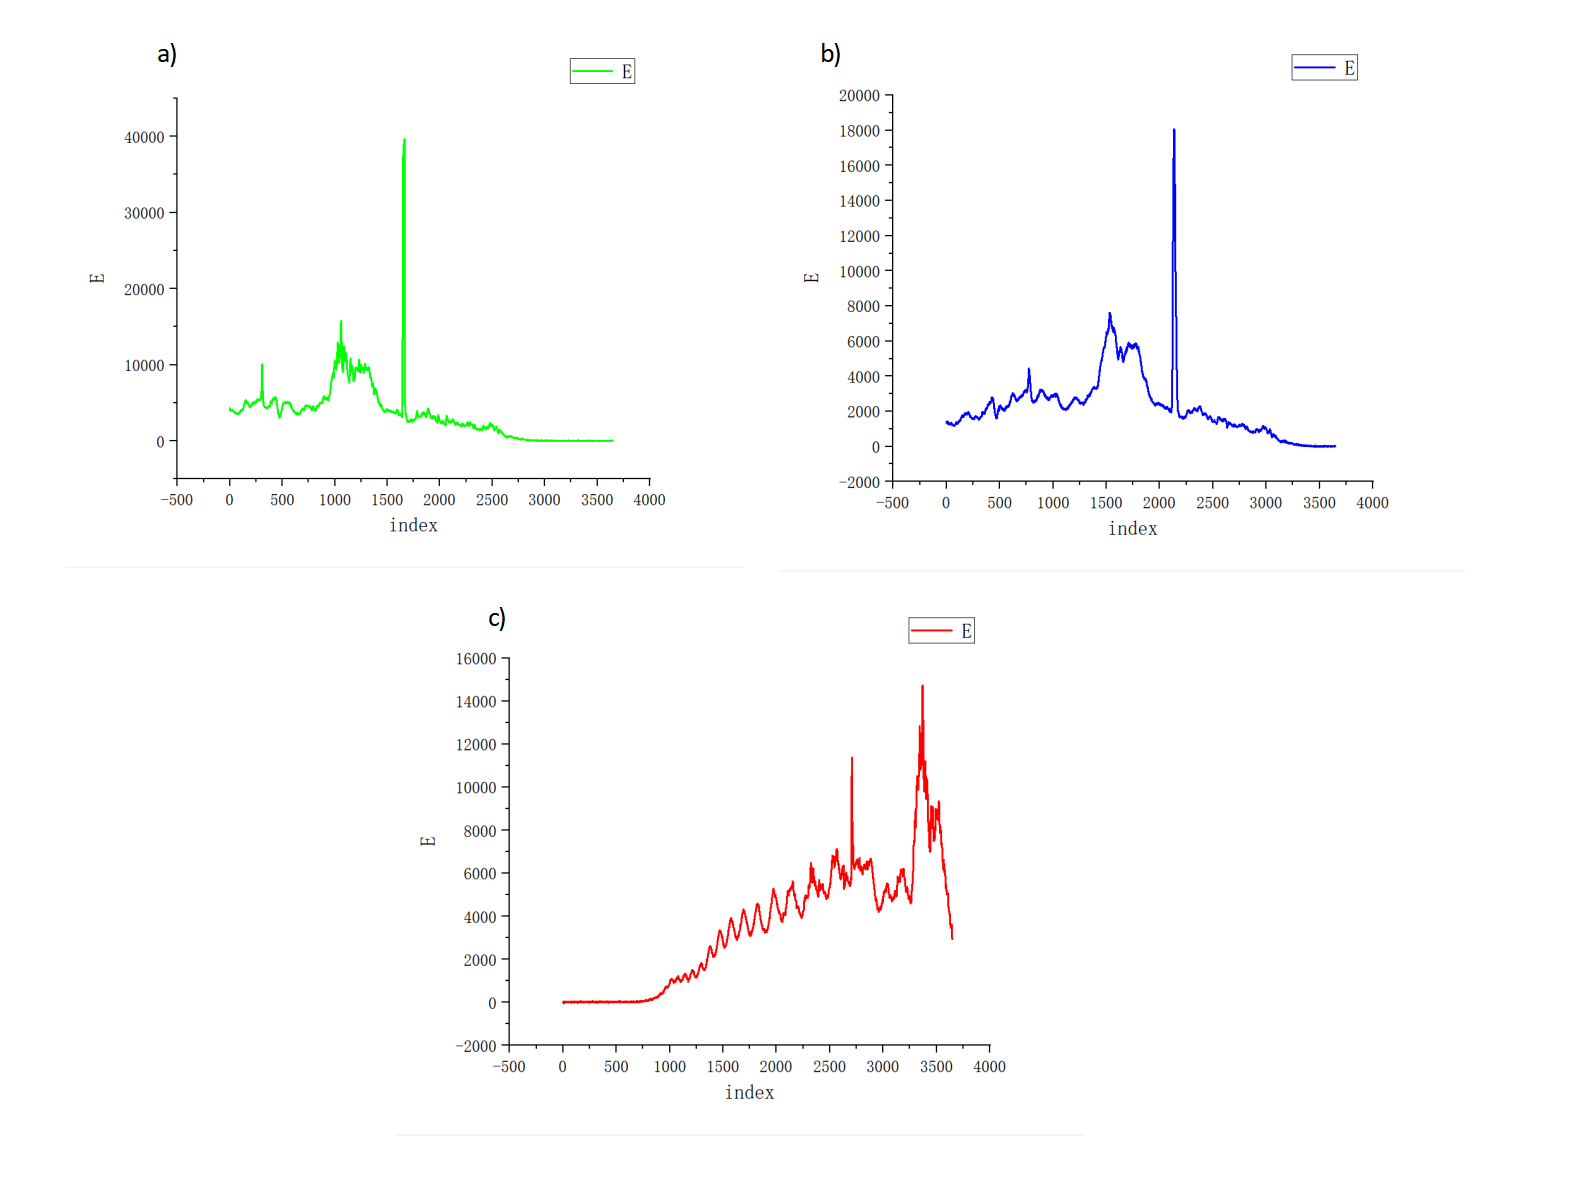
\includegraphics[width=0.7\textwidth]{3.png}
				\bicaption{实验扫描氘灯发射谱图}{Experimental deuterium lamp emission spectrum}
			\end{figure}

			\begin{table}[h]
				\centering
				\zihao{5}
				\bicaption{光谱仪$\lambda$-index数据}{Spectrometer $\lambda$-index data}
				\begin{tabular}{ccccc}
					\toprule
					编号 & $\lambda/{\rm nm}$ & index1 & index2 & index3 \\
					\midrule
					1 	& 485.82 & 728  & 307  & 2707 \\
					2  	& 581.39 & 1529 & 1059 & 3370 \\
					3 	& 656.06 & 2137 & 1664 & None \\
					\bottomrule
				\end{tabular}
			\end{table}
			利用\textbf{表1}数据作散点图如\textbf{图4}所示,可见各点近似落在一条直线上;对$\lambda$-index进行线性拟合,所得回归直线也示于\textbf{图4}中。拟合得到的回归直线表达式分别为:
			$$\lambda / {\rm nm}=-0.1208 \ \ index +397.57,\ \ R=0.99993
			$$
			$$\lambda / {\rm nm}=-0.1255 \ \ index +447.65,\ \ R=0.99997
			$$
			$$\lambda / {\rm nm}=-0.1441 \ \ index +95.61,\ \ R=1
			$$

			\begin{figure}[h]
				\centering
				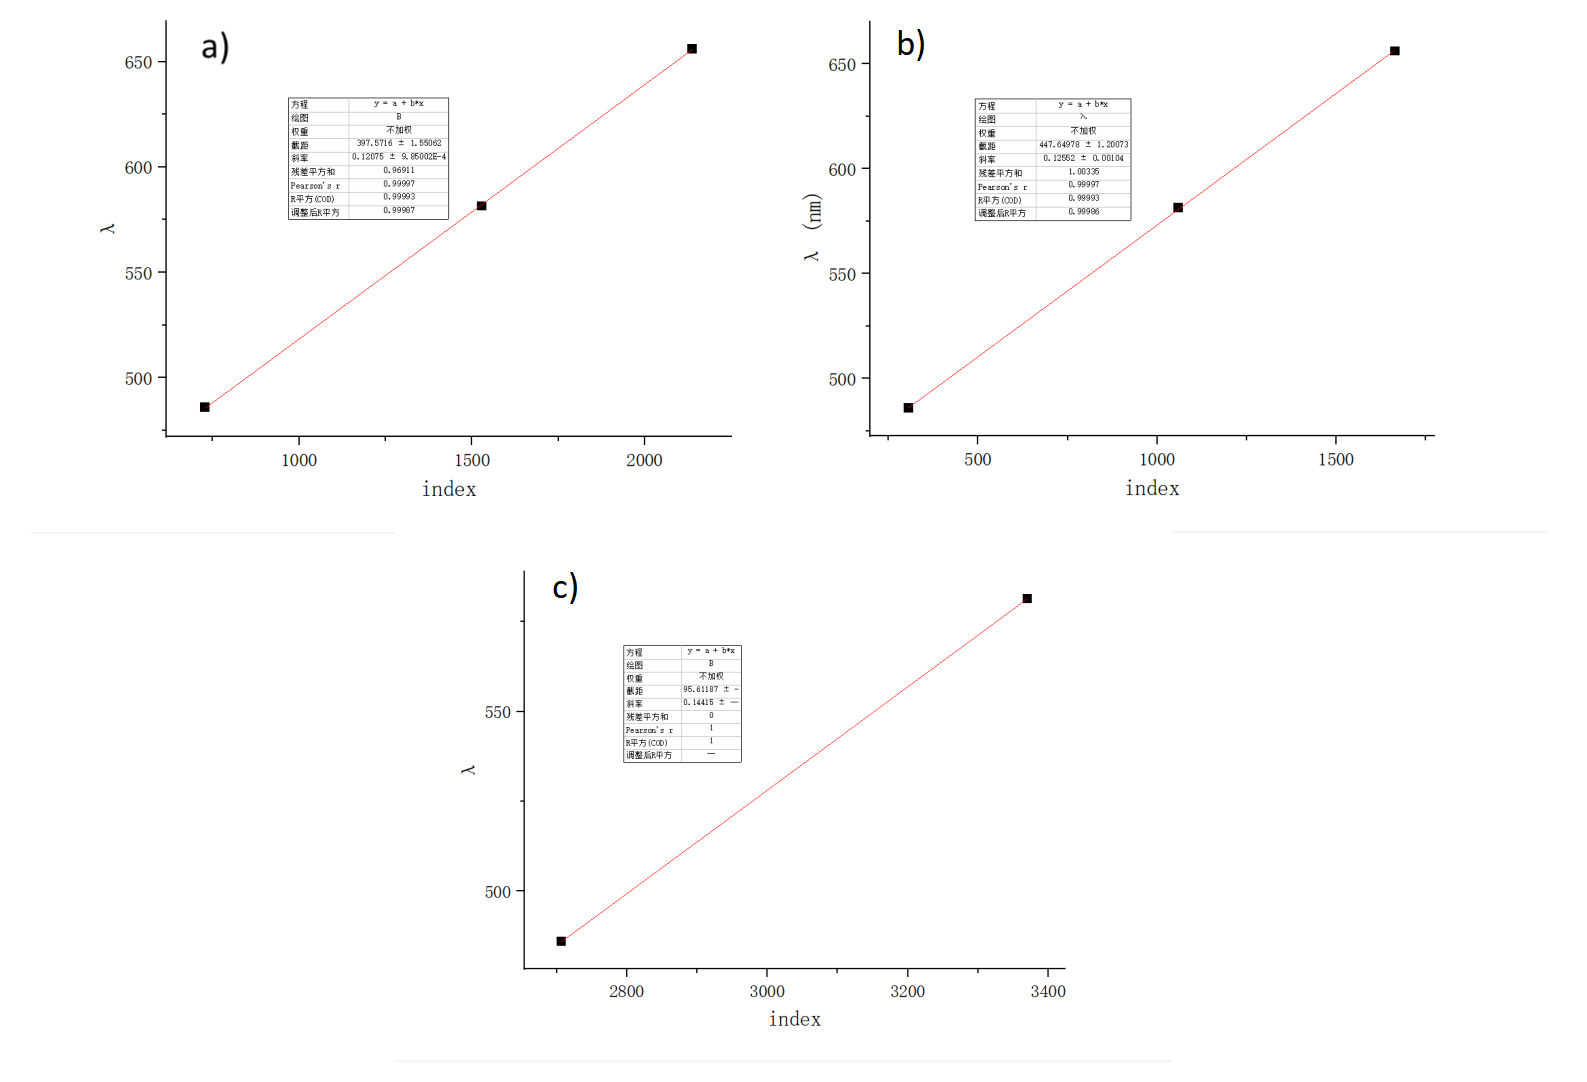
\includegraphics[width=0.65\textwidth]{4.png}
				\bicaption{$\lambda$-index关系图}{Correlation of $\lambda$-index}
			\end{figure}

	 		\subsubsection{测定不同浓度溶液的吸收光谱}
			首先开启卤钨灯,设定积分时间$10\ \ {\rm s}$,采集并扣除暗背景信号。实验室提供了$0.5\ \rm{μmol/L},\ \  1\ \rm{μmol/L}$,\ $5\ \rm{μmol/L},10\ \rm{μmol/L}, \ \ 20\ \rm{μmol/L}, 50\ \rm{μmol/L}$的A3溶液。将各溶液放入样品池中,测量吸收光谱,各溶液的吸收光谱如\textbf{图5}所示:\par

			\begin{figure}[h]
				\centering
				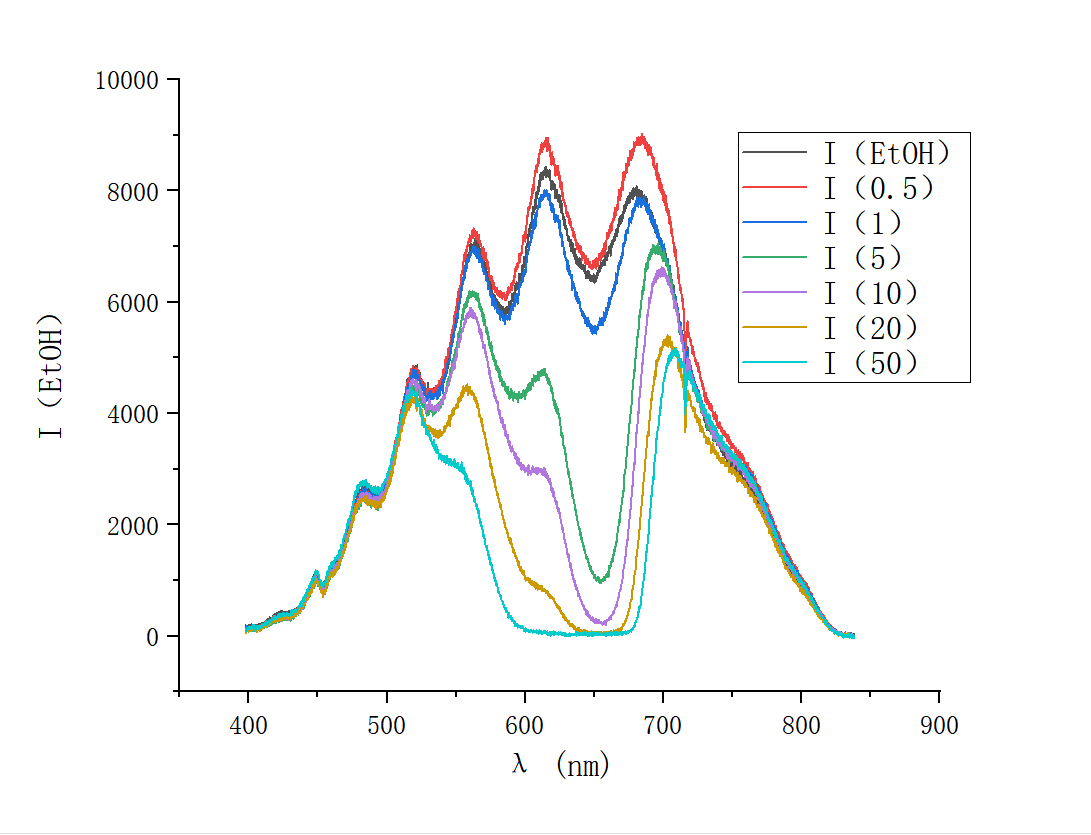
\includegraphics[width=0.6\textwidth]{5.png}
				\bicaption{不同浓度溶液的吸收光谱}{CAbsorption spectra of solutions with different concentrations}
			\end{figure}
			\par

			保存各个样品的透过光强$I$及乙醇的透过光强$I_{0}$,利用公式:\par
			$$
			A=lg(\frac{I_{0}}{I})
			$$
			计算吸光度$A$与波长$\lambda$的关系,结果示于\textbf{图6}。可以看出,三条曲线的主吸收峰位置比较接近,均位于$652.0\ \ {\rm nm}$附近:
			\begin{figure}[h]
				\centering
				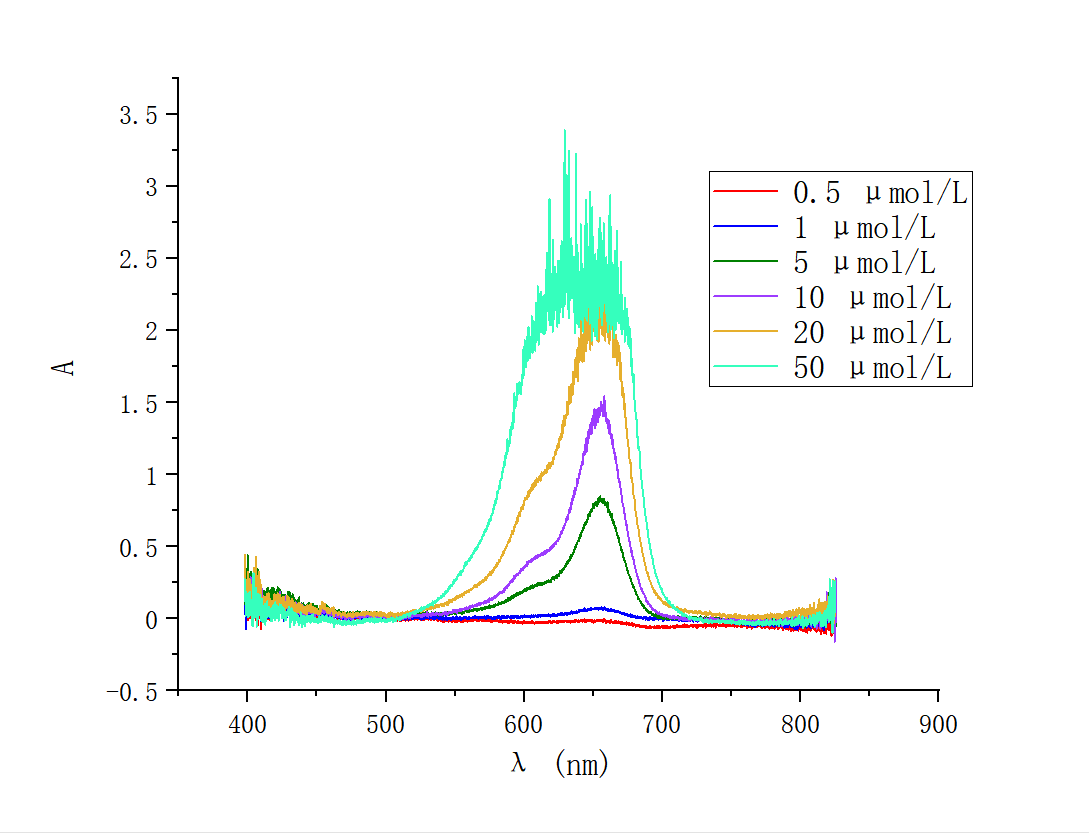
\includegraphics[width=0.70\textwidth]{6.png}
				\bicaption{不同浓度溶液的吸光度曲线}{Absorption curves of solutions with different concentrations}
			\end{figure}
			\par
			从\textbf{图6}和\textbf{图5}可以注意到,在进行作图时我们舍弃了850nm之后的数据,这是因为在850nm之后,各溶液的光强均接近于0,此时信噪比极低,噪声导致的曲线波动极大,且在实际实验中无法通过简单地改变积分时间或对输出取平均值进行有效改善\par
			\subsubsection{Lambert-Beer定律的验证}
			从\textbf{3.1.2}中我们可以注意到,当溶液的浓度提高时,吸收峰的吸收强度增大,且吸收峰的位置不发生明显的变化,这与Lambert-Beer定律的预期相符。
			为了进一步探索Lambert-Beer定律的适用范围,我们对c-A进行线性拟合,如\textbf{图7}所示.\par
			\begin{figure}[h]
				\centering
				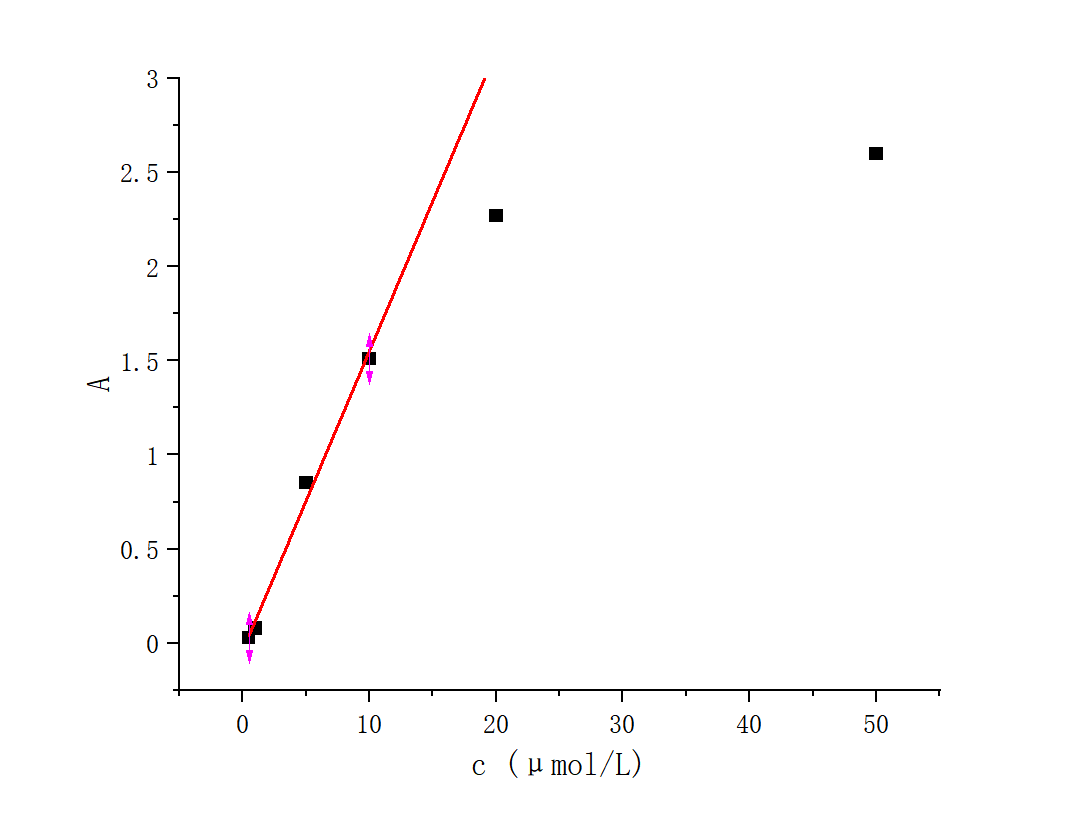
\includegraphics[width=0.6\textwidth]{7.png}
				\bicaption{c-A关系图}{Correlation of A-c}
			\end{figure}

			可以看出,当浓度极小如$0.5\ \rm{μmol/L}$时,此时浓度太低,吸光度太小,无法和噪声区分开,此时的吸光度没有意义。\par
			而当浓度很大时,如$50\ \rm{μmol/L}$时,从\textbf{图6}可以看出吸收峰的吸收强度并没有明显增大,而且吸收曲线变得很抽象,这有可能是因为仪器精度问题,也有可能是因为此时溶液的吸收峰已经接近饱和,无法再吸收更多的光子,因此吸收峰的吸收强度不再增大。
			整体上,当浓度出于$1\sim10\ \rm{μmol/L}$时,吸收峰的吸收强度与浓度成线性关系,且吸收峰的位置不发生明显变化,这与Lambert-Beer定律的预期相符,因此我们认为Lambert-Beer定律在此浓度范围内成立。\par
			
	 		\subsubsection{不同光源下的吸收光谱}
			只开卤钨灯,设定积分时间为$10 {\rm ms}$,测定溶液吸光度曲线;再同时打开氘灯和卤钨灯,设定积分时间为$10 {\rm ms}$,再次测定溶液吸光度曲线,对比示于\textbf{图8}中。\par
			\begin{figure}[h]
				\centering
				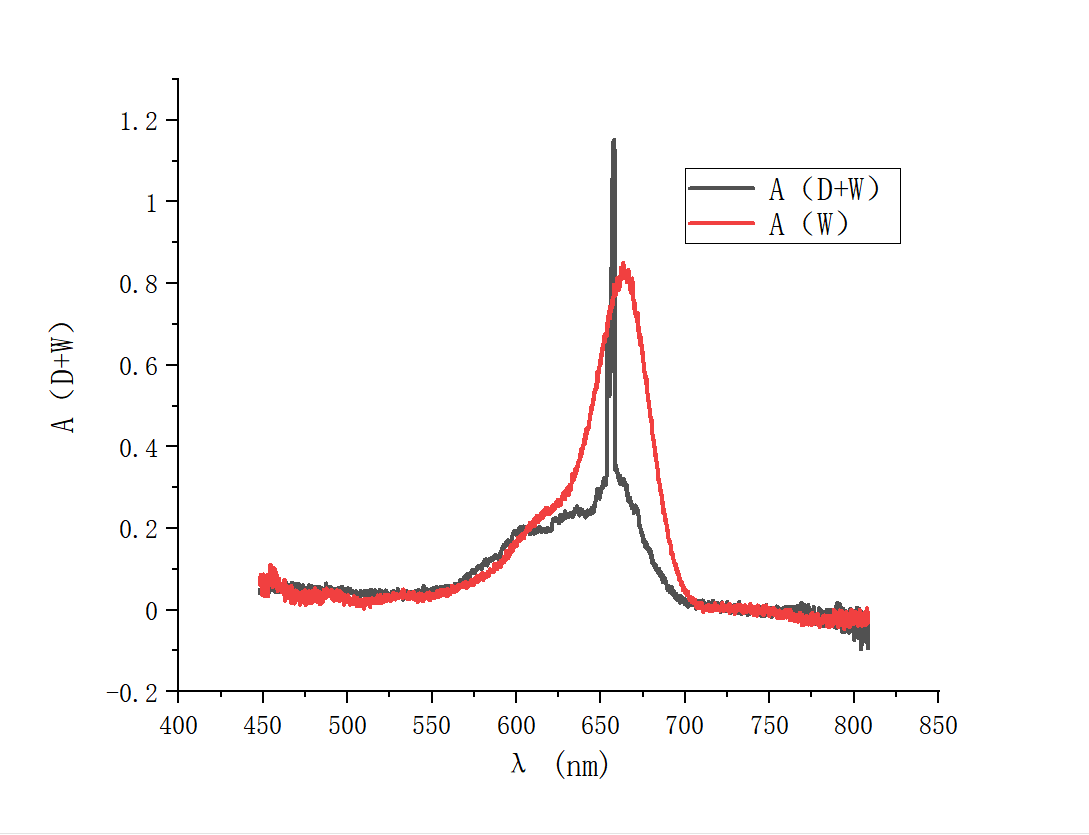
\includegraphics[width=0.6\textwidth]{8.png}
				\bicaption{不同光源下$\rm (A3)$溶液的吸收光谱}{Absorption spectrum of (A) solution under different light sources}
			\end{figure}
			根据\textbf{图8}可以看出,使用氘灯+卤钨灯光源在$\lambda_{max}$处达到了更大的吸光度$A$,但使用卤钨灯光源时吸光度曲线更平滑,信噪比更低,并且基线在0.00附近,相比使用氘灯+卤钨灯光源得到了更合理的结果。在\textbf{图8}中,使用卤钨灯光源和使用氘灯+卤钨灯光源下两条曲线在$\lambda_{max}$处达到了不同的吸光度$A$值,该现象是令人费解的,考虑到Lambert-Beer定律
			$$ A=\varepsilon bc $$
			表明吸光度与光源类型无关;另一个令人费解的现象是当使用氘灯+卤钨光源时吸光度曲线异常尖锐,我们认为这可能是因为${\rm (A3)}$的$\lambda_{max}$在$652.0\ \ {\rm nm}$附近,与氘灯$656.06\ \ {\rm nm}$处的特征峰非常接近,因此使用卤钨灯+氘灯混合光源时,在$\lambda_{max}$处将出现非常尖锐的吸收峰,而氘灯的光强又远强于卤钨灯,因此才会出现\textbf{图8}展示的一个尖锐的大峰加上一个平滑的小峰的结构。\par 
		 	笔者可以理解,使用氘灯+卤钨灯提升信噪比的尝试,但是我们认为这种尝试是失败的,因为使用氘灯+卤钨灯光源时,信噪比并没有明显提升,而且在$\lambda_{max}$处出现了异常的尖锐吸收峰。其根本原因是因为卤钨灯与氘灯的光强差距太大,若光强一致也许会有更好的效果。\par
			
			\subsubsection{各共轭分子的吸收光谱}
			根据各共轭分子溶液的结构大致估测各自$\lambda_{max}$范围,依此在测定吸收光谱的过程中,所有溶液均用卤钨灯光源,积分时间为$10\ \ {\rm ms}$,测得各共轭分子的吸收光谱如\textbf{图9}所示。\par
			这里要首先说明的是,由于实验时间以及ccd接受范围等因素,这一组溶液的的测定并不是在同一时间完成的,仪器的具体位置也不尽相同,这也是为什么\textbf{图9}中各溶液的信噪比不一致的原因。\textbf{图9}是根据标定后的$\lambda$将多组图组合得到的,因此各曲线的起始和终止位置不尽相同,基线也不完全相同的。\par
			\begin{figure}[h]
				\centering
				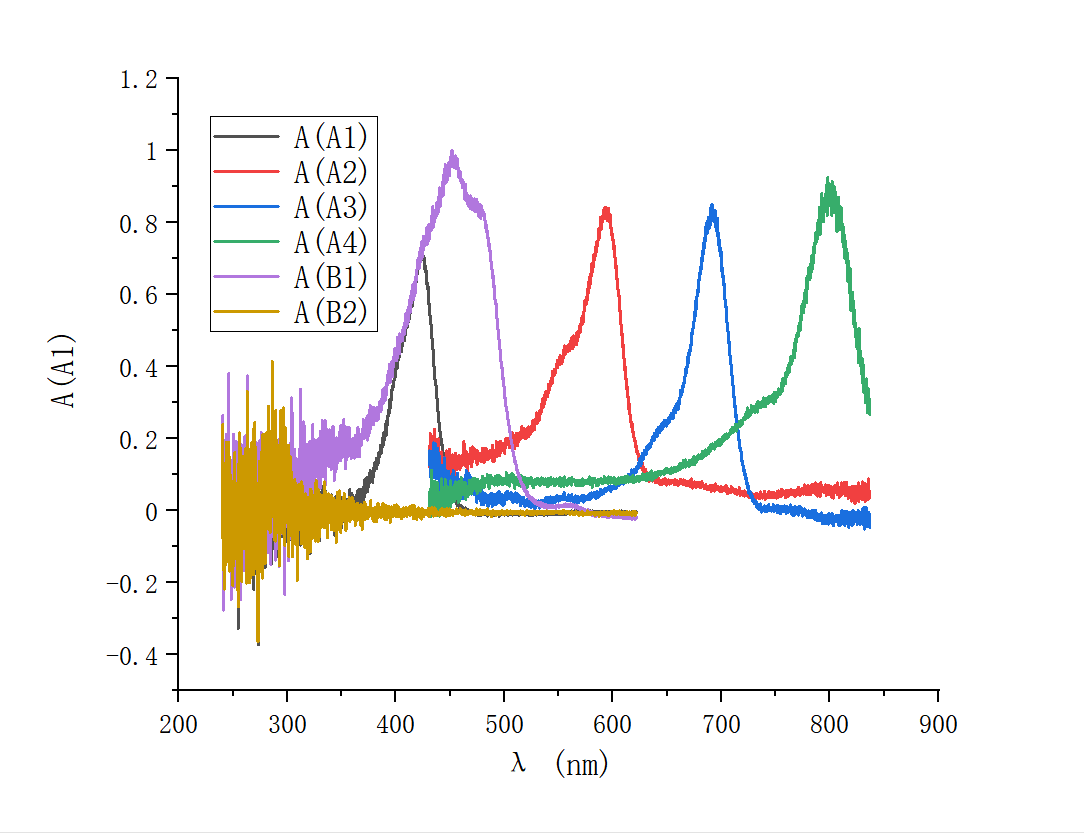
\includegraphics[width=0.65\textwidth]{9.png}
				\bicaption{各共轭分子的吸收光谱}{Absorption spectra of various conjugated molecules}
			\end{figure}
			\par
			对\textbf{图9}使用python matplotlib的自动寻峰功能,可以找到每种分子对应的$\lambda_{max}$,结果如\textbf{表2}所示:\par
			\begin{table}[h]
				\centering
				\zihao{5}
				\bicaption{各共轭分子的最大吸收波长$\lambda_{max}$}{Maximum absorption wavelength $\lambda_{max}$ of various conjugated molecules}
				\begin{tabular}{ccccccc}
					\toprule
					  & A1 & A2 & A3 & A4 & B1 & B2\\
					\midrule
					$\lambda/{\rm nm}$ 	& 424.42 & 563.72  & 652.25  & 761.87 & 451.94 & NAN \\
					\bottomrule
				\end{tabular}
			\end{table}

			其中我们不难注意到,因为卤钨灯在紫外的光强很弱,其在紫外区的信噪比极低,因此吸收在紫外区的分子如A1、B1的吸收曲线会受到很大的影响,而B2更是之没有观测到吸收峰。\par
			因此我们又使用了氘灯光源,重新测量了A1、B1和B2,测得各共轭分子的吸收光谱如\textbf{图10}所示。\par
			\begin{figure}[h]
				\centering
				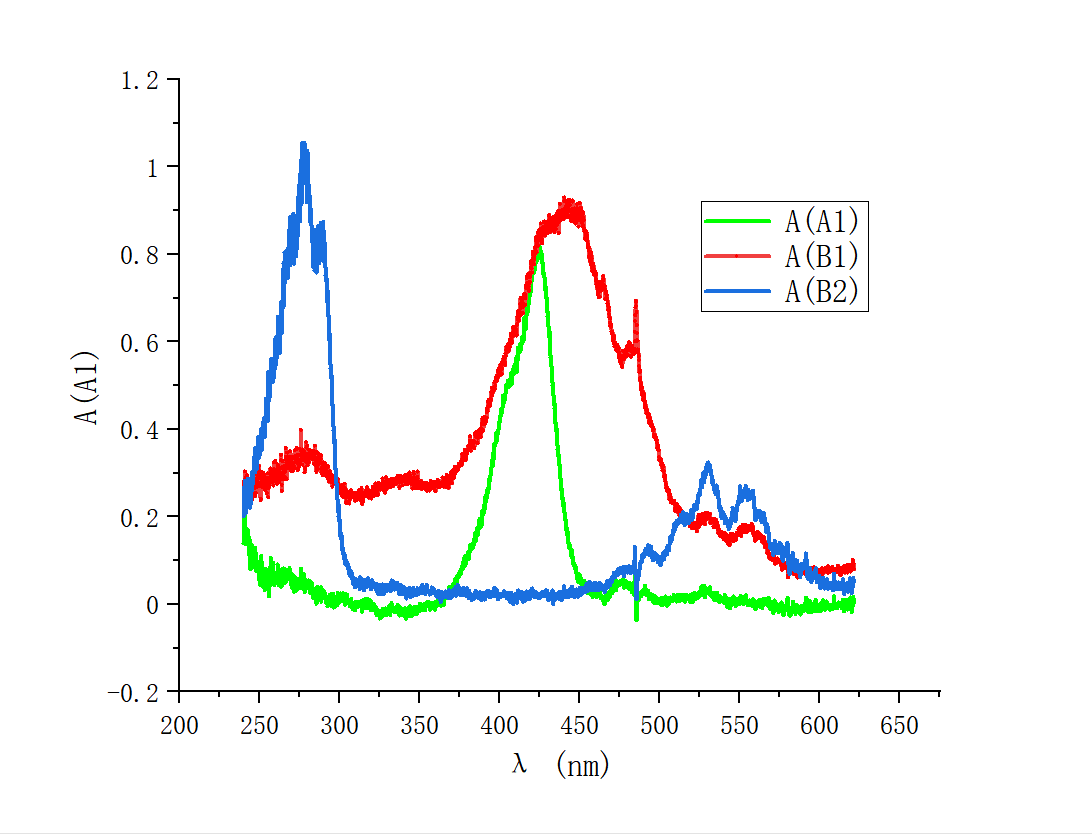
\includegraphics[width=0.6\textwidth]{10.png}
				\bicaption{各共轭分子的吸收光谱}{Absorption spectra of various conjugated molecules}
			\end{figure}
			\par
			对\textbf{图10}使用python matplotlib的自动寻峰功能,可以找到每种分子对应的$\lambda_{max}$,结果如\textbf{表3}所示:\par
			\begin{table}[h]
				\centering
				\zihao{5}
				\bicaption{各共轭分子的最大吸收波长$\lambda_{max}$}{Maximum absorption wavelength $\lambda_{max}$ of various conjugated molecules}
				\begin{tabular}{cccc}
					\toprule
					& A1 & B1 & B2\\
					\midrule
					$\lambda/{\rm nm}$ 	& 424.56 & 441.41 & 277.96 \\
					\bottomrule
				\end{tabular}
			\end{table}
			\par
			可以注意到,换用氘灯后,A1、B1和B2的吸收峰都有了明显的增强,信噪比也有了明显的提升,也成功观测到了B2。但是即使如此,紫外区的信噪比依然较小,一个体现就是紫外区的基线有一个明显的偏移,这也是为什么\textbf{图10}中A1、B1和B2的基线起始不在0.00附近的原因。\par

			\subsection{计算与结果分析}
			\subsubsection{Gaussian理论计算}
			使用GaussView软件搭建$\rm (A)\sim (F)$6个分子,先对分子进行结构优化,将优化后的分子结构作为输入,使用PBE1PBE/6-311g(2d,p)对6个分子进行tddft激发能计算\citealp{ljr};使用GaussView打开结果文件,在Results/UV-Vis中查看结果图谱。
			把理论计算结果与实验测得结果加以比对,计算两种方法得到的$\lambda_{max}$差值,结果示于\textbf{表4}。:
			$$\Delta\lambda_{max}=\lambda_{max, exp}-\lambda_{max, calc}
			$$
			\begin{table}[h]
				\centering
				\zihao{5}
				\bicaption{Gaussian计算与实验测得$\lambda_{max}$的比较}{Comparison of $\lambda_{max}$ obtained by Gaussian calculation and experiment}
				\begin{tabular}{cccc}
					\toprule
					分子  & $\lambda_{max, exp}/{\rm nm} $ & $\lambda_{max, calc} / {\rm nm} $& $\Delta\lambda_{max}/{\rm nm} $  \\
					\midrule
					(A1) & 424.42 & 372.25 & 52.17 \\
					(A2) & 563.72 & 449.89 & 113.83 \\
					(A3) & 652.25 & 503.84 & 148.41 \\
					(A4) & 761.87 & 552.86 & 209.01 \\
					(B1) & 441.41 & 572.61 & -131.20 \\
					(B2) & 277.96 & 300.32 & -22.36\\		
					\bottomrule
				\end{tabular}
			\end{table}
			\par
			根据\textbf{表4}可以看出,Gaussian理论计算在预测本次实验的6个分子的吸收光谱上表现不甚理想,大部分计算值与实验值有明显差别,这可能是使用Gaussian基组对复杂分子进行计算时,大量近似带来的不可忽视的误差导致的。\par
			高斯计算所得的吸收光谱如\textbf{图11}所示:\par
			\begin{figure}[h]
				\centering
				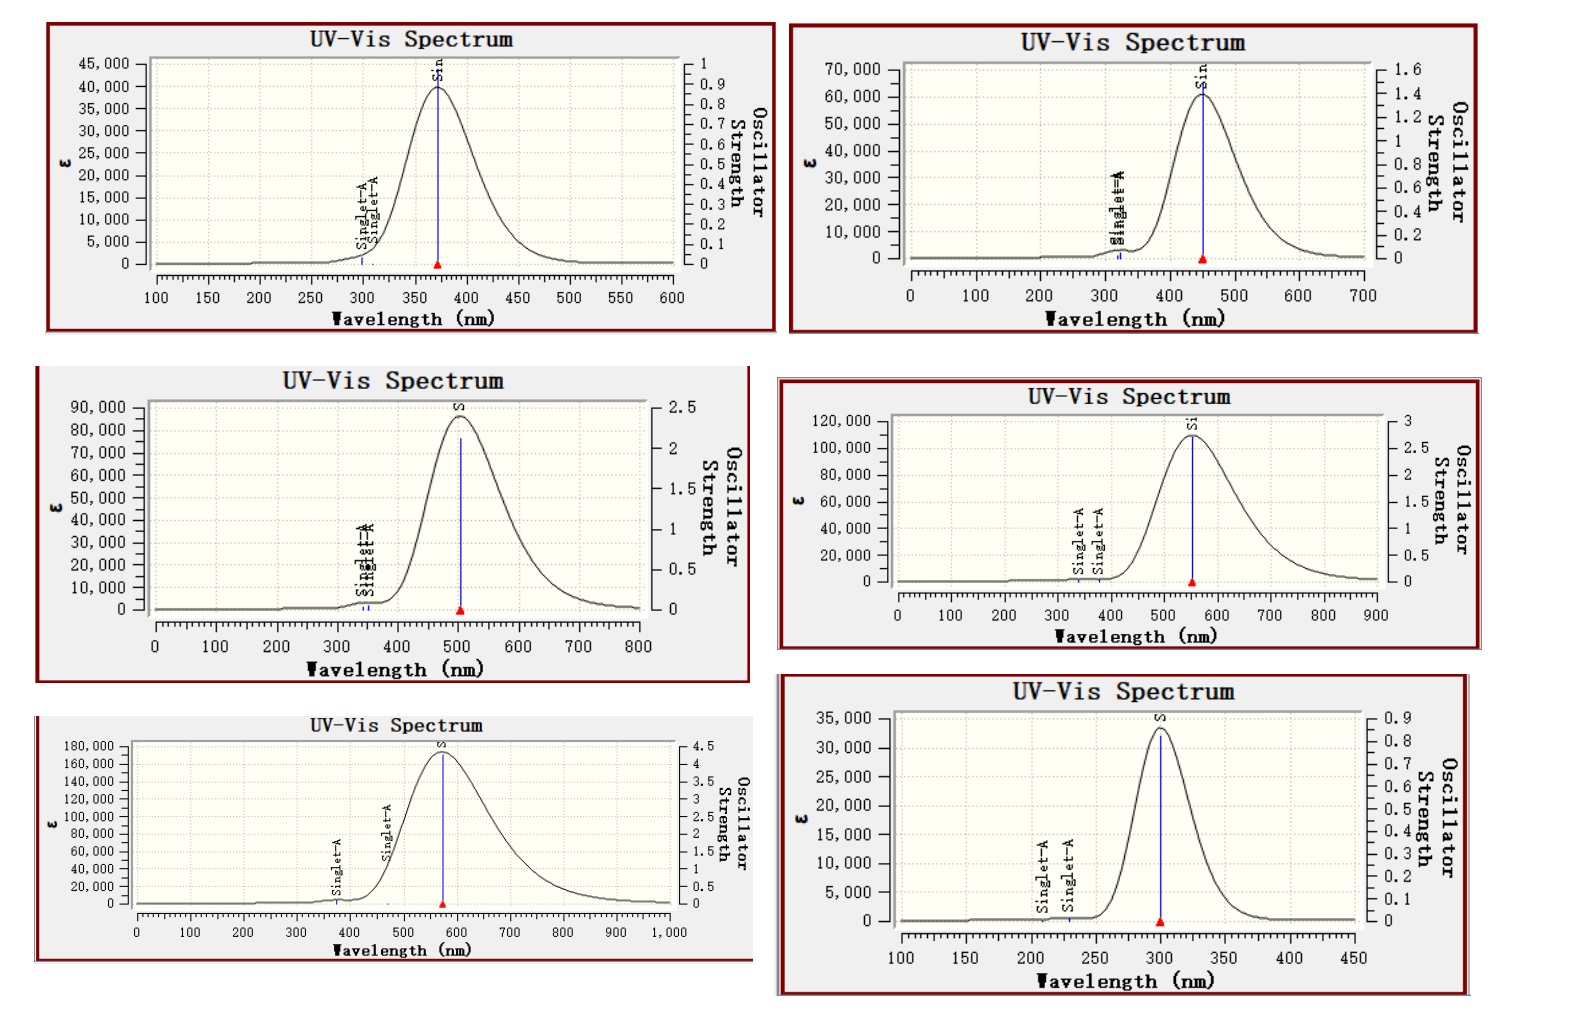
\includegraphics[width=0.65\textwidth]{13.png}
				\bicaption{Gaussian计算与实验测得$\lambda_{max}$的比较}{Comparison of $\lambda_{max}$ obtained by Gaussian calculation and experiment}
			\end{figure}
			\par
			
			\subsubsection{一维势阱模型的验证}
			查询\textit{Lange's Handbook of Chemistry}获得各化学键的键长数据\citealp{dean1992lange},示于\textbf{表5}。
			\begin{table}[h]
				\centering
				\zihao{5}
				\bicaption{各化学键的键长数据}{Bond length data of each chemical bond}
				\begin{tabular}{ccc}
					\toprule
					化学键  & 键长$l/{\rm \AA} $ & 备注  \\
					\midrule
					\ce{C=C} & 1.336 & 共轭双键  \\
					\ce{C-C} & 1.426 & 共轭双键  \\
					\ce{C-C} & 1.395 & 芳环  \\
					\ce{C=N} & 1.320 & 共轭杂环  \\
					\ce{C-N} & 1.353 & 共轭杂环  \\
					\bottomrule
				\end{tabular}
			\end{table}
			\par
			根据一维势阱模型,长度为$L$的势阱中,量子数为$n$的电子能量为:
			$$E=\frac{n^{2}h^{2}}{8mL^{2}}
			$$
			吸收光子从$n$态跃迁到$n+1$态,光子能量等于能级差,有:
			$$\Delta E=\frac{(2n+1)h^{2}}{8mL^{2}}=\frac{hc}{\lambda}
			$$
			故预测吸收光波长:
			$$\lambda=\frac{8mcL^{2}}{(2n+1)h}
			$$
			\par 
			根据\textbf{表5}数据和\textbf{图2}各分子结构,估计一维势阱长度$L$(这里A组分子计算从一端苯环到另一端苯环的距离,B组分子计算共轭体系长度,假设键角为120°),判断量子数$n$,用一维势阱模型计算最大吸收波长$\lambda_{max, quant}$(quant for quantum),并与实验值$\lambda_{max, exp}$对比,相关数据示于\textbf{表6}。
			\begin{table}[h]
				\centering
				\zihao{5}
				\bicaption{一维势阱模型计算$\lambda_{max}$}{Calculation of $\lambda_{max}$ via one-dimensional potential well model}
					\begin{tabular}{ccccc}
						\toprule
						分子  & $\lambda_{max, exp}/{\rm nm} $ & n&$L/{\rm \AA}$ & $\lambda_{max, quant}/{\rm nm} $  \\
						\midrule
						(A1) & 424.42 & 9 & 12.54 & 272.9\\
						(A2) & 563.72 & 10 & 14.94 & 350.4\\
						(A3) & 652.25 & 11 & 17.33 & 430.5\\
						(A4) & 761.87 & 12 & 19.72 & 512.9\\
						(B1) & 441.41 & 10 & 23.91 & 898.0\\
						(B2) & 277.96 & 3 & 7.17 & 242.7\\	
					\bottomrule
				\end{tabular}
			\end{table}
			\par
			\textbf{表6}计算得到的数据与实验值差异异常大,可能的原因一是势阱长度$L$的估计太过粗糙,与真实值差距极大;二是题中所提供的分子具有复杂的平面结构,用一维势阱模型计算本身就是精确度很低的。\par
			我们可以发现,对于共轭体系较小且没有苯环的分子$\rm (B2)$,一维势阱模型计算的结果与实验值相对比较接近,说明一维势阱模型对于该类简单的线性共轭分子是很好的近似;而对于复杂的、具有苯环的平面共轭分子,使用一维势阱模型进行估算会造成很大误差。
			
			
				\section{讨论与结论}
					\subsection{实验讨论}
					\subsubsection{杂质的探究}
					在测量B1和B2时,我们发现除了分子自身的吸收峰外,还有两个较强的吸收峰,其$\lambda_{max}$约为$530\ \ {\rm nm}$和$530\ \ {\rm nm}$,如\textbf{图12}所示:\par
					\begin{figure}[h]
						\centering
						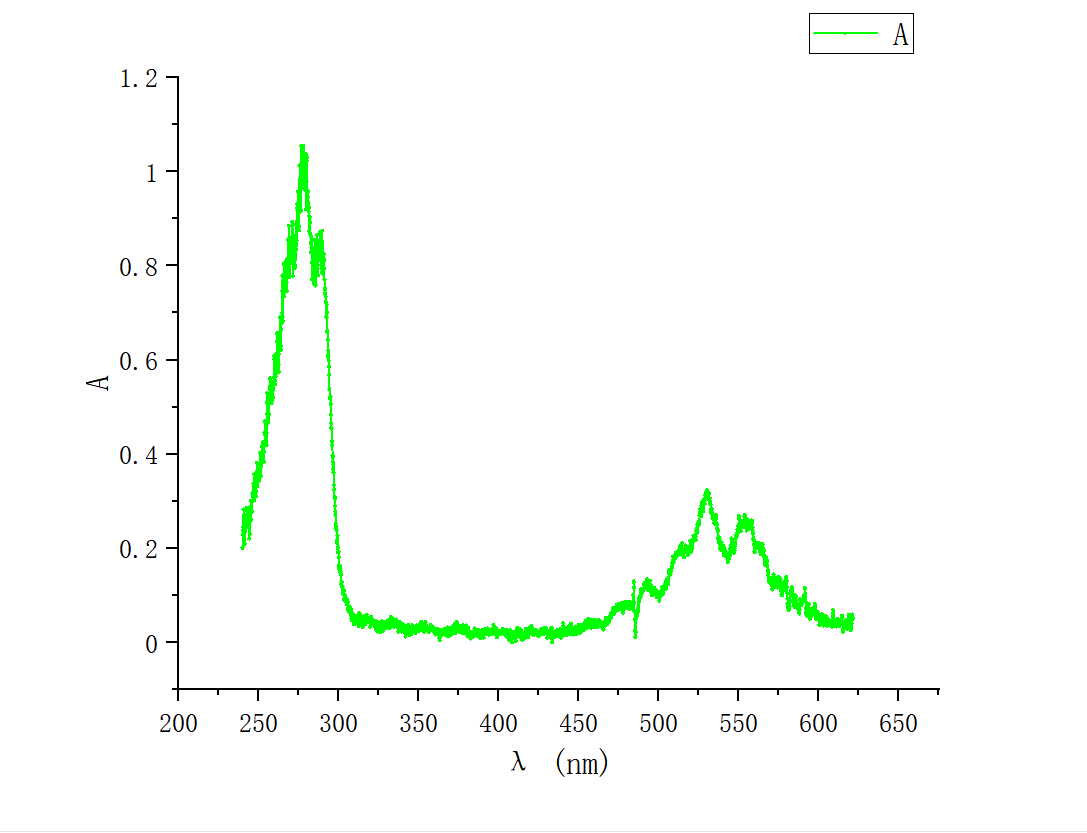
\includegraphics[width=0.6\textwidth]{11.png}
						\bicaption{A3分子的吸收光谱}{Absorption spectra of A3 molecules}
					\end{figure}
					
					起初我们人为这时单次实验的误差,但是在重复测量时,这两个峰的位置始终没有发生变化,我们认为这是因为溶液中存在杂质导致的。但是当我们使用更加专业的仪器测量吸光度时,这两个峰的位置并没有出现,因此我们认为这是因为我们自己组装的仪器存在某些问题,但横向对比其他组的数据,我们发现其他组的数据也存在这两个峰。\par
					从吸收曲线(\textbf{图13})上,我们可以看到测量B2溶液时有明显的在$530\ \ {\rm nm}$-$530\ \ {\rm nm}$区间的吸收,这是在测量其他溶液时没有的现象。笔者不知道为什么会出现这种情况,希望可以在后续讨论等环节解答疑惑.\par
					\begin{figure}[h]
						\centering
						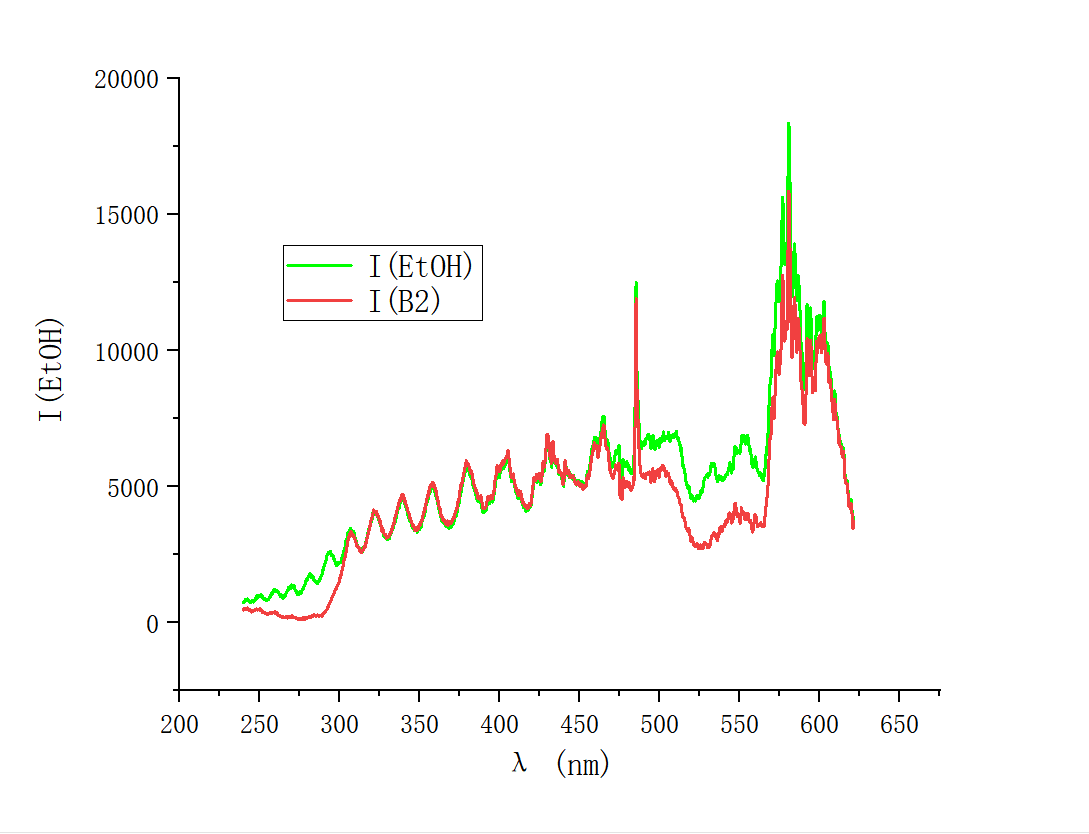
\includegraphics[width=0.7\textwidth]{12.png}
						\bicaption{各共轭分子的吸收光谱}{Absorption spectra of various conjugated molecules}
					\end{figure}
					\par
					\subsubsection{误差分析}
					本次实验中搭建了紫外可见光谱仪,对比了不同浓度和不同分子的吸收光谱,在400~800 nm 的区间内,可以得到与商用光谱仪非常接近的数据,但还是存在一些步骤可能会引入误差,这里对可能引入误差的步骤进行分析:
					\begin{enumerate}
						\item \textbf{搭建仪器}:本次实验中,我们使用的仪器是自己搭建的,因此在搭建仪器的过程中,很多地方无法做到绝对的精确,比如在搭建光路时光路不够直,光路上的镜子不够平整,光线不够平行等等,这些都会引入误差。
						\item \textbf{标定仪器}:在标定仪器时,我们使用的是氘灯,但是氘灯的光强并不是均匀的,ccd的角度以及凹面镜的位置都会影响最终吸收到的光线。同时因为时间缘故,我们的实验分为两周进行,其间温度压强等环境因素都会发生变化,这些都会影响最终的结果。
					\end{enumerate} \par
				  \subsection{实验结论}
			本实验利用实验室提供的器件自主搭建了紫外可见光谱仪,利用氘灯对光谱仪进行标定,确定了$\lambda$-index的线性换算关系。本次实验中搭建了紫外可见光谱仪,对比了不同浓度和不同分子的吸收光谱,在400~800 nm 的区间内,可以得到与商用光谱仪非常接近的数据,但紫外区的信噪比还是偏低。用所搭建的光谱仪测定了同一物质不同浓度的溶液的吸收光谱,观察不同浓度下吸收光谱的差异。对比了氘灯光源和卤钨灯光源的区别,讨论了选取光源的依据。对所给的6个共轭分子的吸收光谱进行了测定,计算了各分子的摩尔消光系数$\varepsilon$。利用Gaussian程序模拟和一维势阱模型对6个共轭分子的吸收光谱或最大吸收波长$\lambda_{max}$进行了计算,比较了计算结果与实验结果的差异,探讨了差异可能的原因。
			 
	\vbox{}
	\section{Supporting Information}
		本实验所有的原始数据、高斯计算文件、shell文件、python代码、实验报告的 LaTeX 源代码均可在 $\rm{https://github.com/wzhstat/Physical\_Chemistry\_Experiments}$找到,原始数据也会邮箱发送给助教。
\vbox{}  
%参考文献
\bibliographystyle{unsrt}
\bibliography{cite}
\end{document}